%----------------------------------------------------------------------------------------
%    PACKAGES AND THEMES
%----------------------------------------------------------------------------------------

\documentclass[aspectratio=169,xcolor=dvipsnames]{beamer}
\usetheme{SimplePlus}

\usepackage{hyperref}
\usepackage{graphicx} % Allows including images
\usepackage{booktabs} % Allows the use of \toprule, \midrule and \bottomrule in tables
\usepackage[T1]{fontenc}
\usepackage{lmodern}
\usepackage[english]{babel}
\usepackage{amsmath, amssymb, mathtools}
\usepackage{xurl} % For better URL line breaking
\usepackage{siunitx}  % For number formatting in tables
\usepackage{emoji}
%----------------------------------------------------------------------------------------
%    TITLE PAGE
%----------------------------------------------------------------------------------------

\title{StyCLIP: StyleTransfer in Few-Shot Learning}
\author{Emanuele Fontana}
\institute{Università degli Studi di Bari Aldo Moro \\ \nolinkurl{e.fontana7@studenti.uniba.it}} % \nolinkurl and manual break if needed
\date{} % Date, can be changed to a custom date

% Define commands from the original paper
\newcommand{\Ft}{\mathbf{F}_\text{t}}      % Text features
\newcommand{\Fv}{\mathbf{F}_\text{v}}      % Visual features (support)
\newcommand{\Wt}{\mathbf{W}_\text{t}}      % Text prototypes
\newcommand{\Wv}{\mathbf{W}_\text{v}}      % Visual prototypes (support)
\newcommand{\fv}{\mathbf{f}_\text{v}}      % Query visual feature
\newcommand{\Figt}{\mathbf{F}_\text{IGT}}  % IGT features
\newcommand{\Ftgi}{\mathbf{F}_\text{TGI}}  % TGI features
\newcommand{\R}{\mathbb{R}}

%----------------------------------------------------------------------------------------
%    PRESENTATION SLIDES
%----------------------------------------------------------------------------------------

\begin{document}

% --- Title Slide ---
\begin{frame}
  \titlepage
\end{frame}



% --- Introduction ---
\section{Introduction}
\begin{frame}
  \frametitle{Introduction \& Motivation}
  \begin{itemize}
    \item \textbf{Context:} Rapid digitization of art collections demands automated artist classification systems for large-scale analysis.
    
    \item \textbf{Challenge:} Few-shot visual artist classification -- identifying artist by their works with limited labeled examples per artist.
    
    \item \textbf{Two Main Goals:}
      \begin{enumerate}
        \item \textbf{Comparative Analysis:} Test different CLIP-based strategies to identify the best approach for few-shot artist classification.
        \item \textbf{Style Enhancement Hypothesis:} Investigate whether explicitly integrating style representations (Gram matrices) into CLIP improves artist-specific pattern recognition.
      \end{enumerate}
    
    \item \textbf{Contribution:} StyCLIP -- a CLIP extension incorporating dedicated style-aware features, evaluated against standard CLIP-based methods.
  \end{itemize}
\end{frame}

% --- Related Work ---
\section{Related Work}
\begin{frame}
  \frametitle{Related Work}
  \begin{block}{Style Transfer}
    \begin{itemize}
        \item Gatys et al. \cite{StyleTransfer}: Deep networks encode style in intermediate layers; Gram matrices capture style.
    \end{itemize}
  \end{block}

  \begin{block}{Few-Shot Learning (FSL) \& Meta-Learning}
    \begin{itemize}
        \item Prototypical Networks \cite{ProtoNet}: Learn to learn from small samples.
    \end{itemize}
  \end{block}

  \begin{block}{Contrastive Language-Image Pretraining (CLIP)}
    \begin{itemize}
        \item CLIP \cite{CLIP}: Shared embedding space for images and text.
        \item TIP-Adapter \cite{TipAdapter}: Cache model for FSL: Zero shot + few-shot classification.
        \item APE \cite{APE}: Adaptive prior refinement of CLIP features.
        \item GDA-CLIP \cite{GDA_CLIP}: Gaussian-based adaptation.
        \item TIMO \cite{TIMO}: Mutual guidance between text/image modalities.
    \end{itemize}
  \end{block}
  \tiny
  % \bibliographystyle{plain} % Use a simple style for beamer - Handled globally at the end
  \nocite{StyleTransfer,ProtoNet,CLIP,TipAdapter,APE,GDA_CLIP,TIMO} % Cite them so they appear
\end{frame}


% --- Dataset ---
\section{Dataset}
\begin{frame}
  \frametitle{Dataset}
  \begin{figure}[H]
    \centering
    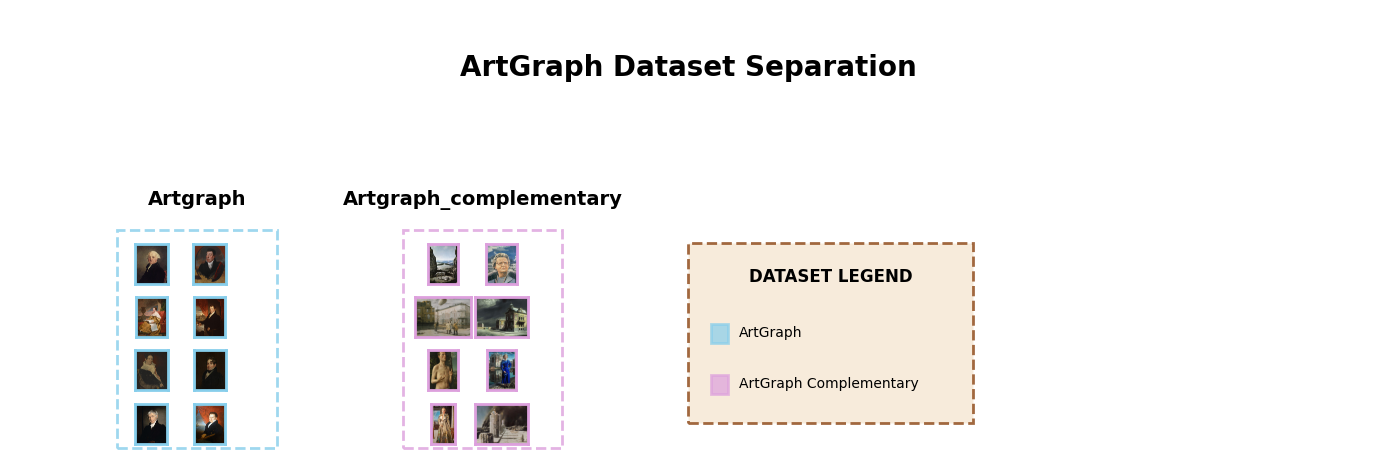
\includegraphics[width=\textwidth ,height=0.75\textheight]{../img/datasets.png}
    \caption{ArtGraph Datasets Overview}
  \end{figure}
  \tiny \nocite{ArtGraph}
\end{frame}




\begin{frame}
  \frametitle{Episode Example for FSL}
  \begin{figure}
    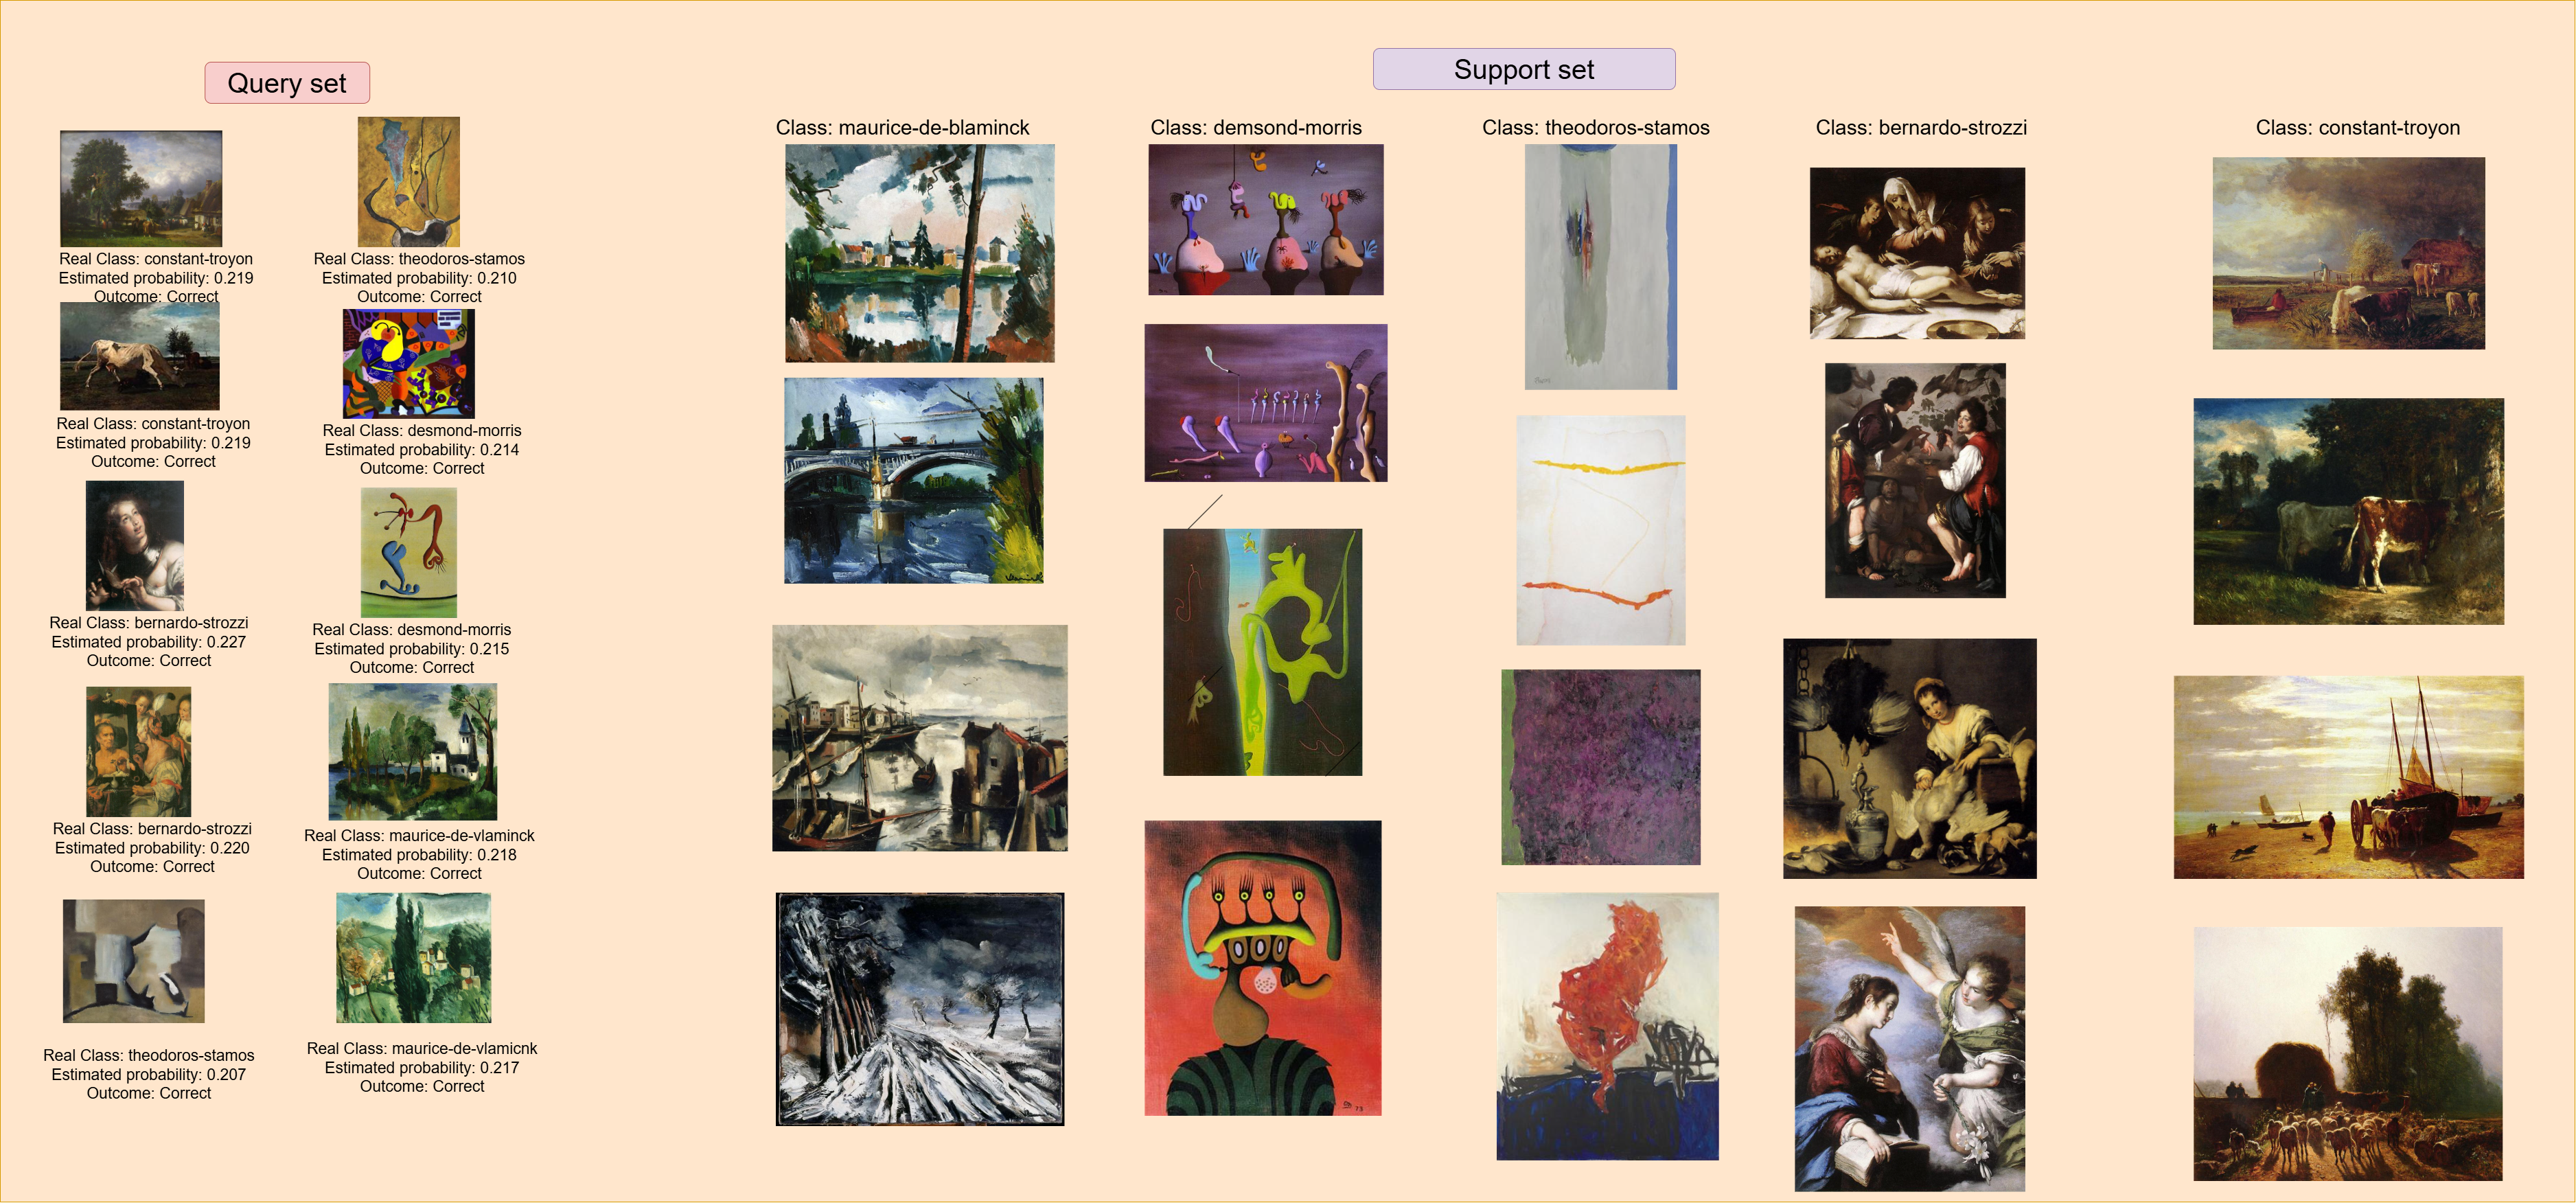
\includegraphics[width=0.8\linewidth,height=0.7\textheight,keepaspectratio]{../img/episode_example.drawio.png} % Adjusted path
    \caption{Example episode: 5-Way, 4-Shots ,10 query examples}
  \end{figure}
\end{frame}

% --- Proposed Method: StyCLIP ---
\section{Our Approach: StyCLIP}
\begin{frame}
  \frametitle{StyCLIP: Architecture Overview}
  \begin{figure}
    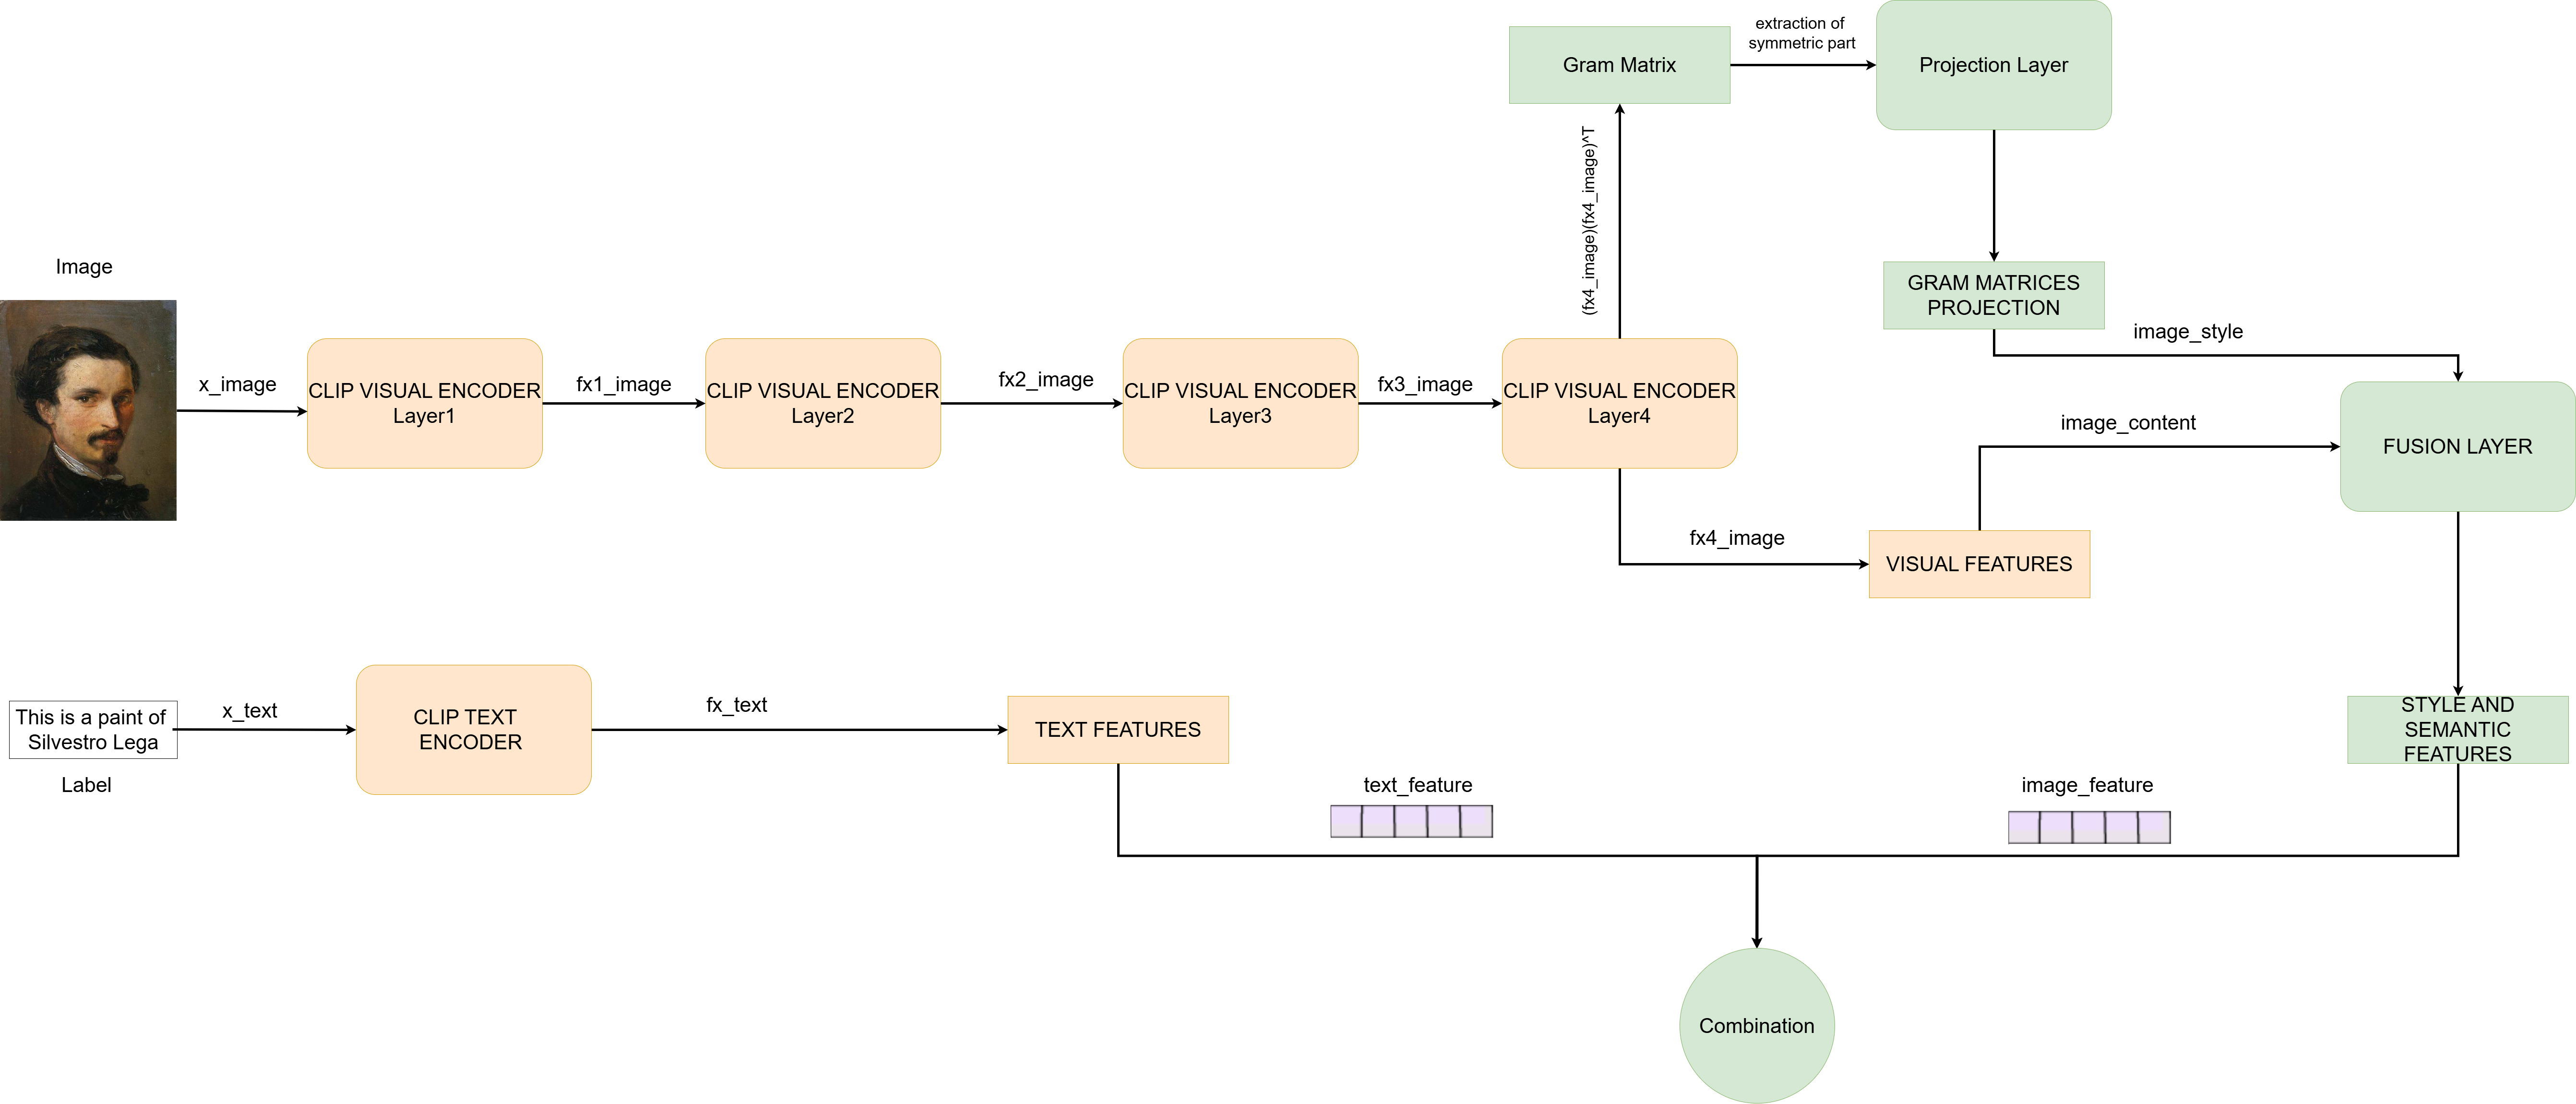
\includegraphics[width=\linewidth,height=0.9\textheight,keepaspectratio]{../img/StyCLIP.png} % Adjusted path
  \end{figure}
\end{frame}

\begin{frame}
  \frametitle{StyCLIP: Key Components}
  \begin{itemize}
    \item \textbf{Three-Stage Architecture:}
      \begin{enumerate}
 \item \textbf{Gram Matrix Extraction:} Extract style correlations from ResNet-50 intermediate layers
        \begin{equation*}
          G_{i,j}^{(l)} = \frac{1}{H \times W} \sum_{k=1}^{H \times W} F_{i,k}^{(l)} \cdot F_{k,j}^{(l)}
        \end{equation*}
        \footnotesize{
        \begin{itemize}
          \item $F^{(l)} \in \R^{C \times H \times W}$: feature maps from layer $l$ (reshaped to $C \times HW$)
          \item $G_{i,j}^{(l)}$: correlation between channels $i$ and $j$ (captures style patterns)
          \item Normalization by $H \times W$ ensures scale-invariance across image sizes
        \end{itemize}
        }
                \item \textbf{Style Projection:} Compress high-dimensional Gram matrices into compact representations
        \begin{equation*}
          \mathbf{s} = \text{MLP}(\text{concat}[\text{vec}(\text{triu}(G^{(2)})), \text{vec}(\text{triu}(G^{(3)}))])
        \end{equation*}
        
        \item \textbf{Adaptive Fusion:} Integrate semantic and style features via bottleneck adapter
        \begin{equation*}
          \mathbf{f}_{\text{fused}} =\text{Adapter}([\Fv; \mathbf{s}])
        \end{equation*}
      \end{enumerate}
      \footnotesize{
        \begin{itemize}
          \item $[\Fv; \mathbf{s}]$: concatenation of CLIP features (512d) and style features (256d)
          \item $\text{Adapter}$: bottleneck MLP ($768 \rightarrow (hyperParamDim) \rightarrow 512$ dimensions)
        \end{itemize}
        }
  \end{itemize}
\end{frame}

\begin{frame}
  \frametitle{StyCLIP: Training Strategy}
  \begin{itemize}
    \item \textbf{Frozen Backbone:} Original CLIP (RN50) visual and text encoders are frozen.
    \item \textbf{Trainable Components:} Only the new style projection layers and fusion adapter are optimized.
    \item \textbf{Rationale:}
      \begin{itemize}
        \item Preserve pre-trained semantic knowledge from CLIP.
        \item Reduce computational cost.
        \item Enable efficient fine-tuning on artistic datasets.
      \end{itemize}
  \end{itemize}

  \begin{block}{Hyperparameter Tuning}
    \begin{itemize}
        \item Optuna \cite{Optuna} used for:
        \begin{itemize}
            \item Fusion bottleneck dimension \{64, 128, 256\}
            \item Dropout rate [0.0, 0.5]
            \item Learning rate log-uniform [$10^{-5}, 10^{-3}$]
            \item Weight decay log-uniform [$10^{-6}, 10^{-3}$]
        \end{itemize}
    \end{itemize}
  \end{block}
  \tiny \nocite{Optuna}
\end{frame}

% --- Experimental Setup ---
\section{Experimental Setup}
\begin{frame}
  \frametitle{Experimental Setup}
  \begin{block}{Meta-Learning Training for StyCLIP}
    \begin{itemize}
      \item Prototypical network approach.
      \item Episodic training: 10-way (N=10 artists), K-shot (K=1, 4) classification, 3-query (Q=3)
    \end{itemize}
  \end{block}

  \begin{block}{Evaluation Protocol}
    \begin{itemize}
      \item \textbf{Method:} Using every CLIP-based method (e.g., TIMO, TIP-Adapter) with every backbone.
      \item N-way classification (all available artists in the test subset).
      \item Tested several times across K $\in \{1, 2, 4, 8, 16\}$ shots for support set.
      \item \textbf{Metrics:} Accuracy, Macro-Precision, Macro-Recall, Macro-F1.
    \end{itemize}
  \end{block}
\end{frame}



% --- Results ---
\section{Results}

\begin{frame}
  \frametitle{Goal 1: Comparative Analysis of CLIP-based Methods}
  \textbf{Best performing combinations for few-shot artist classification:}

  \begin{itemize}
    \item \textbf{TIMO and TIMO-S} emerge as the most effective few-shot learning methods
  \end{itemize}

  \begin{block}{Top Performers: 16-Shot Classification Accuracy (\%)}
    \centering
    \tiny
    \begin{tabular}{@{}lcc@{}}
      \toprule
      \textbf{Method} & \textbf{Backbone} & \textbf{Accuracy (\%)} \\
      \midrule
      \textbf{TIMO-S}    & \textbf{RN50} & \textbf{73.46} \\
      \textbf{TIMO}      & \textbf{RN50} & \textbf{73.36} \\
      GDA-CLIP  & RN50 & 73.06 \\
      APE       & RN50 & 62.17 \\
      TIP-Adapter & RN50 & 52.91 \\
      \bottomrule
    \end{tabular}
    \normalsize
  \end{block}
  
  \textbf{Key Finding:} TIMO-based methods with RN50 backbone achieve optimal performance for few-shot artist classification.
\end{frame}

\begin{frame}
  \frametitle{Goal 2: Style Enhancement Hypothesis - Results}
  \textbf{Hypothesis:} Explicit style representations (Gram matrices) improve artist classification.
  
  \textbf{Result:} Hypothesis \textbf{rejected} - StyCLIP consistently underperforms standard CLIP variants.

  \begin{block}{StyCLIP vs Standard CLIP: 16-Shot Accuracy (\%)}
    \centering
    \tiny
    \begin{tabular}{@{}lccc@{}}
      \toprule
      \textbf{Method} & \textbf{RN50} & \textbf{StyCLIP\_FSL1} & \textbf{StyCLIP\_FSL4} \\
      \midrule
      TIMO-S    & \textbf{73.46} & 39.20 & 48.75 \\
      TIMO      & \textbf{73.36} & 37.00 & 43.27 \\
      GDA-CLIP  & \textbf{73.06} & 41.19 & 53.36 \\
      APE       & \textbf{62.17} & 6.73  & 7.98  \\
      \bottomrule
    \end{tabular}
    \normalsize
  \end{block}
  \begin{itemize}
    \item \textbf{Performance Gap:} Standard RN50 outperforms best StyCLIP variant by $\sim$25 percentage points
    \item \textbf{Statistical Significance:} T-tests confirm significant differences (p < 0.05)
    \item \textbf{Consistency:} Pattern holds across all shot configurations (1, 2, 4, 8, 16)
  \end{itemize}
\end{frame}

\begin{frame}
  \frametitle{Performance Analysis Across Shot Configurations}
  \begin{figure}[H]
    \centering
    \tiny
    \begin{tabular}{@{}lcc@{}}
      \toprule
      \textbf{Shot Config} & \textbf{TIMO-S + RN50} & \textbf{TIMO-S + StyCLIP\_FSL4} \\
      \midrule
      1-shot  & 45.96\% & 7.31\%  \\
      2-shot  & 48.65\% & 15.38\% \\
      4-shot  & 57.28\% & 26.36\% \\
      8-shot  & 65.08\% & 40.89\% \\
      16-shot & 73.46\% & 48.75\% \\
      \bottomrule
    \end{tabular}
  \end{figure}
    \begin{itemize}
    \item Both approaches improve with more support examples
    \item \textbf{Performance gap persists} across all configurations
  \end{itemize}
\end{frame}


% --- Conclusion ---
\section{Conclusion \& Discussion}
\begin{frame}
  \frametitle{Conclusion \& Discussion}
  \begin{itemize}
    \item \textbf{Main Finding:} Integrating explicit style-aware features via Gram matrices (StyCLIP) did \textbf{not improve} few-shot artist classification performance.
    \item \textbf{Implication:} Explicit Gram matrix-based style modeling might interfere with CLIP's pre-trained semantic representations rather than enhance them for this task.
    \item \textbf{Future Directions:} Alternative approaches like attention-based style integration or domain-specific fine-tuning (without architectural changes) might be more fruitful.
  \end{itemize}
\end{frame}

% --- Acknowledgments & Code ---
\section{Acknowledgments \& Code}

% --- Acknowledgments & Code ---
\section{Acknowledgments \& Code}
\begin{frame}
  \frametitle{Acknowledgments and Code}
  \begin{itemize}
    \item This work was proposed by PhD student \textbf{Nicola Fanelli} and \textbf{Prof. Giovanna Castellano} at the University of Bari
  \item The code for this project is available on GitHub:
  \begin{center}
    \url{https://github.com/Fonty02/ComputerVision/tree/main/TIMO}
  \end{center}
  \vspace{2em} % Use \vspace for vertical spacing in Beamer
  \begin{center}
    \Large Thank You! \emoji{rocket}
  \end{center}
    \end{itemize}
\end{frame}

%-------------------------------------------------
%    APPENDIX
%-------------------------------------------------
\appendix
\section{Appendix}

\begin{frame}
  \frametitle{Appendix: Hyperparameter Optimization Highlights}
  \begin{columns}[T] % Use T for top alignment if preferred, or c for center
    \begin{column}{0.5\textwidth}
      \begin{block}{StyCLIP FSL1 (1-shot trained)}
        \begin{itemize}
          \item Bottleneck: 64
          \item LR: $6.01 \times 10^{-5}$
          \item Dropout: 0.0
          \item Weight Decay: $4.83 \times 10^{-4}$
          \item Valid Acc: 57.07\%
        \end{itemize}
      \end{block}
    \end{column}
    \begin{column}{0.5\textwidth}
      \begin{block}{StyCLIP FSL4 (4-shot trained)}
        \begin{itemize}
          \item Bottleneck: 128
          \item LR: $1.02 \times 10^{-5}$
          \item Dropout: 0.1
          \item Weight Decay: $1.03 \times 10^{-6}$
          \item Valid Acc: 60.53\%
        \end{itemize}
      \end{block}
    \end{column}
  \end{columns}
\end{frame}


%------------------------------------------------
%    REFERENCES
%------------------------------------------------
\begin{frame}[allowframebreaks]
    \frametitle{References}
    \footnotesize % SimplePlus theme might handle this, but can be kept
    \bibliography{bibo}
    \bibliographystyle{plain} % Changed from apalike to plain as in presCV.tex
\end{frame}

%----------------------------------------------------------------------------------------
%    THE END
%----------------------------------------------------------------------------------------
\begin{frame}
    \Huge{\centerline{\textbf{The End}}}
\end{frame}

\end{document}